%% FreqODES project report -- Elsevier CAS single-column template (cas-sc)
%% Compile on Overleaf (template "Elsevier's CAS LaTeX Single Column") or locally:
%%   pdflatex main && bibtex main && pdflatex main && pdflatex main
\documentclass[a4paper,fleqn]{cas-sc}
\usepackage[T1]{fontenc}
\usepackage{lmodern}
\usepackage[numbers]{natbib}
\usepackage{booktabs,multirow,graphicx,amsmath,xcolor}
\usepackage{tikz}
\usetikzlibrary{arrows.meta,positioning,fit,backgrounds}

% Remove the template's left footer ("<short authors>: Preprint submitted to Elsevier"); keep "Page x of y"
\ExplSyntaxOn
\cs_set:Npn \__first_footerline: {}
\ExplSyntaxOff

\newcommand{\DBNKTennoDW}{78.48}
\newcommand{\JBNKTennoDW}{--}
\newcommand{\TBNKTennoDW}{176}
\newcommand{\DBNKTennoDWLiver}{87.71}
\newcommand{\JBNKTennoDWLiver}{--}
\newcommand{\DBNKTennoDWLK}{75.86}
\newcommand{\JBNKTennoDWLK}{--}
\newcommand{\DBNKTennoDWRK}{73.33}
\newcommand{\JBNKTennoDWRK}{--}
\newcommand{\DBNKTennoDWSpleen}{77.01}
\newcommand{\JBNKTennoDWSpleen}{--}
\newcommand{\DBNKTen}{78.38}
\newcommand{\JBNKTen}{--}
\newcommand{\TBNKTen}{176}
\newcommand{\DBNKTenLiver}{87.70}
\newcommand{\JBNKTenLiver}{--}
\newcommand{\DBNKTenLK}{75.59}
\newcommand{\JBNKTenLK}{--}
\newcommand{\DBNKTenRK}{73.51}
\newcommand{\JBNKTenRK}{--}
\newcommand{\DBNKTenSpleen}{76.71}
\newcommand{\JBNKTenSpleen}{--}
\newcommand{\DBNKFifty}{79.26}
\newcommand{\JBNKFifty}{--}
\newcommand{\TBNKFifty}{181}
\newcommand{\DBNKFiftyLiver}{87.82}
\newcommand{\JBNKFiftyLiver}{--}
\newcommand{\DBNKFiftyLK}{76.99}
\newcommand{\JBNKFiftyLK}{--}
\newcommand{\DBNKFiftyRK}{74.71}
\newcommand{\JBNKFiftyRK}{--}
\newcommand{\DBNKFiftySpleen}{77.51}
\newcommand{\JBNKFiftySpleen}{--}
\newcommand{\DDWTKTen}{77.33}
\newcommand{\JDWTKTen}{--}
\newcommand{\TDWTKTen}{116}
\newcommand{\DDWTKTenLiver}{86.92}
\newcommand{\JDWTKTenLiver}{--}
\newcommand{\DDWTKTenLK}{74.47}
\newcommand{\JDWTKTenLK}{--}
\newcommand{\DDWTKTenRK}{71.95}
\newcommand{\JDWTKTenRK}{--}
\newcommand{\DDWTKTenSpleen}{75.99}
\newcommand{\JDWTKTenSpleen}{--}
\newcommand{\DDWTKFifty}{78.97}
\newcommand{\JDWTKFifty}{--}
\newcommand{\TDWTKFifty}{120}
\newcommand{\DDWTKFiftyLiver}{87.69}
\newcommand{\JDWTKFiftyLiver}{--}
\newcommand{\DDWTKFiftyLK}{76.68}
\newcommand{\JDWTKFiftyLK}{--}
\newcommand{\DDWTKFiftyRK}{74.16}
\newcommand{\JDWTKFiftyRK}{--}
\newcommand{\DDWTKFiftySpleen}{77.34}
\newcommand{\JDWTKFiftySpleen}{--}
\newcommand{\DFFTKTen}{77.31}
\newcommand{\JFFTKTen}{--}
\newcommand{\TFFTKTen}{116}
\newcommand{\DFFTKTenLiver}{86.69}
\newcommand{\JFFTKTenLiver}{--}
\newcommand{\DFFTKTenLK}{73.43}
\newcommand{\JFFTKTenLK}{--}
\newcommand{\DFFTKTenRK}{72.21}
\newcommand{\JFFTKTenRK}{--}
\newcommand{\DFFTKTenSpleen}{76.93}
\newcommand{\JFFTKTenSpleen}{--}
\newcommand{\DFFTKFifty}{79.34}
\newcommand{\JFFTKFifty}{--}
\newcommand{\TFFTKFifty}{123}
\newcommand{\DFFTKFiftyLiver}{87.89}
\newcommand{\JFFTKFiftyLiver}{--}
\newcommand{\DFFTKFiftyLK}{77.39}
\newcommand{\JFFTKFiftyLK}{--}
\newcommand{\DFFTKFiftyRK}{74.63}
\newcommand{\JFFTKFiftyRK}{--}
\newcommand{\DFFTKFiftySpleen}{77.43}
\newcommand{\JFFTKFiftySpleen}{--}
\newcommand{\DFREQKTennoDW}{77.30}
\newcommand{\JFREQKTennoDW}{--}
\newcommand{\TFREQKTennoDW}{116}
\newcommand{\DFREQKTennoDWLiver}{86.71}
\newcommand{\JFREQKTennoDWLiver}{--}
\newcommand{\DFREQKTennoDWLK}{74.45}
\newcommand{\JFREQKTennoDWLK}{--}
\newcommand{\DFREQKTennoDWRK}{72.19}
\newcommand{\JFREQKTennoDWRK}{--}
\newcommand{\DFREQKTennoDWSpleen}{75.86}
\newcommand{\JFREQKTennoDWSpleen}{--}
\newcommand{\DFREQKTen}{77.65}
\newcommand{\JFREQKTen}{--}
\newcommand{\TFREQKTen}{117}
\newcommand{\DFREQKTenLiver}{86.79}
\newcommand{\JFREQKTenLiver}{--}
\newcommand{\DFREQKTenLK}{74.53}
\newcommand{\JFREQKTenLK}{--}
\newcommand{\DFREQKTenRK}{72.26}
\newcommand{\JFREQKTenRK}{--}
\newcommand{\DFREQKTenSpleen}{77.03}
\newcommand{\JFREQKTenSpleen}{--}
\newcommand{\DFREQKFifty}{78.91}
\newcommand{\JFREQKFifty}{--}
\newcommand{\TFREQKFifty}{123}
\newcommand{\DFREQKFiftyLiver}{87.76}
\newcommand{\JFREQKFiftyLiver}{--}
\newcommand{\DFREQKFiftyLK}{76.67}
\newcommand{\JFREQKFiftyLK}{--}
\newcommand{\DFREQKFiftyRK}{73.96}
\newcommand{\JFREQKFiftyRK}{--}
\newcommand{\DFREQKFiftySpleen}{77.24}
\newcommand{\JFREQKFiftySpleen}{--}
\newcommand{\DFUSEDKTenLQuarter}{78.11}
\newcommand{\JFUSEDKTenLQuarter}{--}
\newcommand{\TFUSEDKTenLQuarter}{178}
\newcommand{\DFUSEDKTenLQuarterLiver}{87.24}
\newcommand{\JFUSEDKTenLQuarterLiver}{--}
\newcommand{\DFUSEDKTenLQuarterLK}{75.29}
\newcommand{\JFUSEDKTenLQuarterLK}{--}
\newcommand{\DFUSEDKTenLQuarterRK}{73.34}
\newcommand{\JFUSEDKTenLQuarterRK}{--}
\newcommand{\DFUSEDKTenLQuarterSpleen}{76.56}
\newcommand{\JFUSEDKTenLQuarterSpleen}{--}
\newcommand{\DFUSEDKTenLFifty}{78.15}
\newcommand{\JFUSEDKTenLFifty}{--}
\newcommand{\TFUSEDKTenLFifty}{178}
\newcommand{\DFUSEDKTenLFiftyLiver}{87.03}
\newcommand{\JFUSEDKTenLFiftyLiver}{--}
\newcommand{\DFUSEDKTenLFiftyLK}{75.41}
\newcommand{\JFUSEDKTenLFiftyLK}{--}
\newcommand{\DFUSEDKTenLFiftyRK}{72.97}
\newcommand{\JFUSEDKTenLFiftyRK}{--}
\newcommand{\DFUSEDKTenLFiftySpleen}{77.19}
\newcommand{\JFUSEDKTenLFiftySpleen}{--}
\newcommand{\DFUSEDKTenLThreeQ}{77.98}
\newcommand{\JFUSEDKTenLThreeQ}{--}
\newcommand{\TFUSEDKTenLThreeQ}{179}
\newcommand{\DFUSEDKTenLThreeQLiver}{87.04}
\newcommand{\JFUSEDKTenLThreeQLiver}{--}
\newcommand{\DFUSEDKTenLThreeQLK}{75.90}
\newcommand{\JFUSEDKTenLThreeQLK}{--}
\newcommand{\DFUSEDKTenLThreeQRK}{72.44}
\newcommand{\JFUSEDKTenLThreeQRK}{--}
\newcommand{\DFUSEDKTenLThreeQSpleen}{76.55}
\newcommand{\JFUSEDKTenLThreeQSpleen}{--}
\newcommand{\DFUSEDKFiftyLFifty}{79.35}
\newcommand{\JFUSEDKFiftyLFifty}{--}
\newcommand{\TFUSEDKFiftyLFifty}{183}
\newcommand{\DFUSEDKFiftyLFiftyLiver}{87.84}
\newcommand{\JFUSEDKFiftyLFiftyLiver}{--}
\newcommand{\DFUSEDKFiftyLFiftyLK}{77.29}
\newcommand{\JFUSEDKFiftyLFiftyLK}{--}
\newcommand{\DFUSEDKFiftyLFiftyRK}{74.59}
\newcommand{\JFUSEDKFiftyLFiftyRK}{--}
\newcommand{\DFUSEDKFiftyLFiftySpleen}{77.68}
\newcommand{\JFUSEDKFiftyLFiftySpleen}{--}
\newcommand{\DODESK}{79.26}
\newcommand{\JODESK}{--}
\newcommand{\TODESK}{125}
\newcommand{\DODESKLiver}{87.74}
\newcommand{\JODESKLiver}{--}
\newcommand{\DODESKLK}{77.28}
\newcommand{\JODESKLK}{--}
\newcommand{\DODESKRK}{74.72}
\newcommand{\JODESKRK}{--}
\newcommand{\DODESKSpleen}{77.32}
\newcommand{\JODESKSpleen}{--}
\newcommand{\DRANDOMKTennoDW}{78.19}
\newcommand{\JRANDOMKTennoDW}{--}
\newcommand{\TRANDOMKTennoDW}{115}
\newcommand{\DRANDOMKTennoDWLiver}{87.57}
\newcommand{\JRANDOMKTennoDWLiver}{--}
\newcommand{\DRANDOMKTennoDWLK}{75.27}
\newcommand{\JRANDOMKTennoDWLK}{--}
\newcommand{\DRANDOMKTennoDWRK}{73.20}
\newcommand{\JRANDOMKTennoDWRK}{--}
\newcommand{\DRANDOMKTennoDWSpleen}{76.71}
\newcommand{\JRANDOMKTennoDWSpleen}{--}
\newcommand{\DRANDOMKTen}{78.15}
\newcommand{\JRANDOMKTen}{--}
\newcommand{\TRANDOMKTen}{115}
\newcommand{\DRANDOMKTenLiver}{87.49}
\newcommand{\JRANDOMKTenLiver}{--}
\newcommand{\DRANDOMKTenLK}{75.36}
\newcommand{\JRANDOMKTenLK}{--}
\newcommand{\DRANDOMKTenRK}{73.33}
\newcommand{\JRANDOMKTenRK}{--}
\newcommand{\DRANDOMKTenSpleen}{76.44}
\newcommand{\JRANDOMKTenSpleen}{--}
\newcommand{\DRANDOMKFifty}{79.21}
\newcommand{\JRANDOMKFifty}{--}
\newcommand{\TRANDOMKFifty}{120}
\newcommand{\DRANDOMKFiftyLiver}{87.61}
\newcommand{\JRANDOMKFiftyLiver}{--}
\newcommand{\DRANDOMKFiftyLK}{77.26}
\newcommand{\JRANDOMKFiftyLK}{--}
\newcommand{\DRANDOMKFiftyRK}{74.31}
\newcommand{\JRANDOMKFiftyRK}{--}
\newcommand{\DRANDOMKFiftySpleen}{77.67}
\newcommand{\JRANDOMKFiftySpleen}{--}
\newcommand{\Dsourceonly}{64.29}
\newcommand{\Jsourceonly}{--}
\newcommand{\Tsourceonly}{53}
\newcommand{\DsourceonlyLiver}{84.17}
\newcommand{\JsourceonlyLiver}{--}
\newcommand{\DsourceonlyLK}{47.28}
\newcommand{\JsourceonlyLK}{--}
\newcommand{\DsourceonlyRK}{52.94}
\newcommand{\JsourceonlyRK}{--}
\newcommand{\DsourceonlySpleen}{72.76}
\newcommand{\JsourceonlySpleen}{--}
\newcommand{\PFFTKTen}{0.009}
\newcommand{\DiffFFTKTen}{-1.06}
\newcommand{\PDWTKTen}{0.005}
\newcommand{\DiffDWTKTen}{-1.05}
\newcommand{\PFREQKTen}{0.044}
\newcommand{\DiffFREQKTen}{-0.73}
\newcommand{\PFUSEDKTenLFifty}{0.469}
\newcommand{\DiffFUSEDKTenLFifty}{-0.23}
\newcommand{\PRANDOMKTen}{0.573}
\newcommand{\DiffRANDOMKTen}{-0.22}
\newcommand{\PFFTKFifty}{0.748}
\newcommand{\DiffFFTKFifty}{+0.08}
\newcommand{\PDWTKFifty}{0.136}
\newcommand{\DiffDWTKFifty}{-0.29}
\newcommand{\PFREQKFifty}{0.070}
\newcommand{\DiffFREQKFifty}{-0.35}
\newcommand{\PFUSEDKFiftyLFifty}{0.629}
\newcommand{\DiffFUSEDKFiftyLFifty}{+0.09}
\newcommand{\PRANDOMKFifty}{0.904}
\newcommand{\DiffRANDOMKFifty}{-0.05}
\newcommand{\AUCFFT}{0.994}
\newcommand{\AUCDWT}{0.969}
\newcommand{\AUCFREQ}{0.993}

\newcommand{\VBnTenMean}{78.31}
\newcommand{\VBnTenStd}{1.38}
\newcommand{\VBnTenDiff}{+0.00}
\newcommand{\VBnTenP}{1.000}
\newcommand{\VBnTenIoU}{65.51}
\newcommand{\VBnTenTime}{154}
\newcommand{\VBnTenSa}{76.80}
\newcommand{\VBnTenSb}{78.67}
\newcommand{\VBnTenSc}{79.48}
\newcommand{\VFqTenMean}{78.54}
\newcommand{\VFqTenStd}{0.13}
\newcommand{\VFqTenDiff}{+0.22}
\newcommand{\VFqTenP}{0.908}
\newcommand{\VFqTenIoU}{65.63}
\newcommand{\VFqTenTime}{104}
\newcommand{\VFqTenSa}{78.39}
\newcommand{\VFqTenSb}{78.62}
\newcommand{\VFqTenSc}{78.61}
\newcommand{\VFvTenMean}{78.66}
\newcommand{\VFvTenStd}{0.26}
\newcommand{\VFvTenDiff}{+0.35}
\newcommand{\VFvTenP}{0.199}
\newcommand{\VFvTenIoU}{65.84}
\newcommand{\VFvTenTime}{105}
\newcommand{\VFvTenSa}{78.36}
\newcommand{\VFvTenSb}{78.80}
\newcommand{\VFvTenSc}{78.82}
\newcommand{\VFaTenMean}{78.36}
\newcommand{\VFaTenStd}{0.28}
\newcommand{\VFaTenDiff}{+0.04}
\newcommand{\VFaTenP}{0.700}
\newcommand{\VFaTenIoU}{65.57}
\newcommand{\VFaTenTime}{104}
\newcommand{\VFaTenSa}{78.30}
\newcommand{\VFaTenSb}{78.11}
\newcommand{\VFaTenSc}{78.66}
\newcommand{\VFeTenMean}{79.11}
\newcommand{\VFeTenStd}{0.17}
\newcommand{\VFeTenDiff}{+0.80}
\newcommand{\VFeTenP}{0.004}
\newcommand{\VFeTenIoU}{66.43}
\newcommand{\VFeTenTime}{104}
\newcommand{\VFeTenSa}{78.93}
\newcommand{\VFeTenSb}{79.16}
\newcommand{\VFeTenSc}{79.26}
\newcommand{\VRdTenMean}{78.29}
\newcommand{\VRdTenStd}{0.57}
\newcommand{\VRdTenDiff}{-0.02}
\newcommand{\VRdTenP}{0.232}
\newcommand{\VRdTenIoU}{65.40}
\newcommand{\VRdTenTime}{102}
\newcommand{\VRdTenSa}{78.84}
\newcommand{\VRdTenSb}{77.70}
\newcommand{\VRdTenSc}{78.33}
\newcommand{\VBnFiftyMean}{79.40}
\newcommand{\VBnFiftyStd}{0.18}
\newcommand{\VBnFiftyDiff}{+0.00}
\newcommand{\VBnFiftyP}{1.000}
\newcommand{\VBnFiftyIoU}{66.90}
\newcommand{\VBnFiftyTime}{163}
\newcommand{\VBnFiftySa}{79.20}
\newcommand{\VBnFiftySb}{79.50}
\newcommand{\VBnFiftySc}{79.50}
\newcommand{\VFqFiftyMean}{79.04}
\newcommand{\VFqFiftyStd}{0.15}
\newcommand{\VFqFiftyDiff}{-0.36}
\newcommand{\VFqFiftyP}{0.000}
\newcommand{\VFqFiftyIoU}{66.36}
\newcommand{\VFqFiftyTime}{109}
\newcommand{\VFqFiftySa}{78.87}
\newcommand{\VFqFiftySb}{79.08}
\newcommand{\VFqFiftySc}{79.17}
\newcommand{\VFvFiftyMean}{78.91}
\newcommand{\VFvFiftyStd}{0.27}
\newcommand{\VFvFiftyDiff}{-0.49}
\newcommand{\VFvFiftyP}{0.000}
\newcommand{\VFvFiftyIoU}{66.18}
\newcommand{\VFvFiftyTime}{109}
\newcommand{\VFvFiftySa}{78.61}
\newcommand{\VFvFiftySb}{78.98}
\newcommand{\VFvFiftySc}{79.14}
\newcommand{\VFeFiftyMean}{79.13}
\newcommand{\VFeFiftyStd}{0.33}
\newcommand{\VFeFiftyDiff}{-0.27}
\newcommand{\VFeFiftyP}{0.018}
\newcommand{\VFeFiftyIoU}{66.44}
\newcommand{\VFeFiftyTime}{104}
\newcommand{\VFeFiftySa}{78.75}
\newcommand{\VFeFiftySb}{79.35}
\newcommand{\VFeFiftySc}{79.28}
\newcommand{\VRdFiftyMean}{79.10}
\newcommand{\VRdFiftyStd}{0.23}
\newcommand{\VRdFiftyDiff}{-0.30}
\newcommand{\VRdFiftyP}{0.001}
\newcommand{\VRdFiftyIoU}{66.43}
\newcommand{\VRdFiftyTime}{107}
\newcommand{\VRdFiftySa}{78.86}
\newcommand{\VRdFiftySb}{79.11}
\newcommand{\VRdFiftySc}{79.31}


% ---------------- GROUP DETAILS (edit) ----------------
\newcommand{\GroupName}{Group A12}
% -------------------------------------------------------

\tikzset{
  blk/.style={draw, rounded corners=2pt, minimum height=7mm, align=center, font=\scriptsize, fill=#1!15},
  blk/.default=gray,
  arr/.style={-{Stealth[length=2mm]}, thick},
  new/.style={draw=red!70!black, very thick, dashed, rounded corners=3pt}
}

\begin{document}
\let\WriteBookmarks\relax
\def\floatpagepagefraction{1}
\def\textpagefraction{.001}

\shorttitle{FreqODES: frequency-guided online active domain adaptation}
\shortauthors{\GroupName}

\title [mode = title]{FreqODES: Frequency-domain guided online domain adaptation with expert-in-the-loop active learning for abdominal MRI segmentation}

\author[1]{Vishnu Vardhan (CB.SC.U4AIE23043)}
\author[1]{Nithya Sai (CB.SC.U4AIE23021)}
\affiliation[1]{organization={Amrita School of Artificial Intelligence, Amrita Vishwa Vidyapeetham},
    addressline={22AIE437 Medical Image Processing, \GroupName},
    country={India}}

\begin{abstract}
Segmentation networks trained on one MR sequence degrade when deployed on another. ODES (MICCAI 2025) adapts a pre-trained network online, patient by patient, by asking an expert to label 1\% of the pixels of a pruned subset of slices and updating only the batch-normalisation (BN) layers. Its image-pruning step ranks slices by the KL divergence between BN statistics of the source model and of augmented copies of each slice. We reproduce ODES on CHAOS T1-DUAL in-phase$\rightarrow$out-of-phase MRI after completing the public code (training script, missing diversity module, device and selection fixes), obtaining a mean Dice of \DODESK\% with all slices annotated (paper: 78.61\%) and \DBNKTen\% with 10\% of slices (paper: 76.80\%). We then propose FreqODES, which replaces the network-internal score by an interpretable frequency-domain shift score built from FFT radial-band energies and Haar wavelet sub-band energies, optionally fused with the BN score. The frequency score separates source from target slices with ROC-AUC \AUCFFT\ and requires no forward passes, reducing the online adaptation time by about one third, but used alone it does not beat ODES: a good detector of domain shift is not necessarily a good detector of annotation value. Guided by this analysis, the final method, FreqODES-U, multiplies the frequency shift by the model's prediction uncertainty. Over three seeds, with 10\% of slices annotated, it reaches \VFeTenMean\% mean Dice against \VBnTenMean\% for ODES ($\Delta=\VFeTenDiff$, $p=\VFeTenP$, paired Wilcoxon over 60 patient-runs), with a seed-to-seed standard deviation of \VFeTenStd\ instead of \VBnTenStd\ and a one-third shorter adaptation pass; with 50\% of slices ODES remains slightly better (\VBnFiftyMean\% vs.\ \VFeFiftyMean\%).
\end{abstract}

\begin{keywords}
Online domain adaptation \sep Active learning \sep Test-time adaptation \sep Fourier transform \sep Wavelet transform \sep MRI segmentation \sep CHAOS
\end{keywords}

\maketitle

\section{Introduction}
Automatic segmentation of the liver, kidneys and spleen in abdominal MRI supports surgical planning, organ volumetry and longitudinal follow-up. Convolutional networks achieve high accuracy when training and test images come from the same scanner and sequence, but their accuracy drops when the acquisition changes---the \emph{domain shift} problem. Even within a single examination, the in-phase (IP) and out-of-phase (OOP) echoes of a T1-weighted dual gradient-echo sequence look different: OOP images show chemical-shift cancellation artefacts at fat--water boundaries and a different texture, and a model trained on IP images loses more than ten Dice points on OOP images (Section~\ref{sec:results}).

Retraining for every new site requires expert annotations, which are slow and expensive. Test-time adaptation methods such as TENT~\cite{wang2021tent} adapt without labels by minimising prediction entropy, but pseudo-labels are unreliable in safety-critical settings. ODES~\cite{islam2025odes} combines the two worlds: the model is adapted online, one patient at a time, using a very small expert budget chosen by active learning. Its first step, \emph{image pruning}, decides which slices are worth the expert's time by measuring their domain shift through batch-normalisation statistics.

This report has two goals. First, we \textbf{replicate} ODES on the CHAOS IP$\rightarrow$OOP benchmark and compare with the published numbers. Second, we \textbf{modify} the pruning step: motivated by the observation that sequence and scanner shifts appear directly in the spatial-frequency content of an image~\cite{yang2020fda}, we replace the BN score with a frequency-domain score computed with the Fast Fourier Transform (FFT) and the Discrete Wavelet Transform (DWT)~\cite{mallat1989wavelet}. Our contributions are:
\begin{itemize}
  \item a complete, runnable replication of ODES, including the components missing from the public repository;
  \item FreqODES, an interpretable, forward-pass-free FFT/DWT domain-shift score and its fusion with the BN score;
  \item an analysis of why the shift score alone does not improve annotation selection, and FreqODES-U, which combines frequency shift with model uncertainty and outperforms ODES at a 10\% slice budget over three seeds;
  \item controlled comparisons at equal annotation budgets with ablations and paired statistical tests, reporting every evaluated variant.
\end{itemize}

\section{Base paper and replication}
\subsection{ODES}
ODES~\cite{islam2025odes} (Islam et al., MICCAI 2025) considers a source-trained segmentation network $f_\theta$ that receives a stream of target batches $X_1,X_2,\dots$; in MRI one batch is the stack of 2-D slices of one patient. For every batch it (i) predicts pseudo-labels, (ii) prunes the batch to the $K\%$ most shifted slices, (iii) selects square patches covering $b\%$ of each kept slice for expert labelling, and (iv) updates the BN affine parameters with a cross-entropy loss on the labelled pixels, after which the next patient is processed (Fig.~\ref{fig:arch}).

\paragraph{Image pruning.} Each slice $x_j$ is augmented (flips, rotations) and the augmented copies are passed through a copy of the network whose BN layers record batch statistics. Assuming Gaussian channel activations, the divergence from the source statistics is
\begin{equation}
D_{BN}(x_j)=\sum_{l}\sum_{c}\mathrm{KL}\!\left[\mathcal{N}(\mu^S_{lc},\sigma^{S\,2}_{lc})\,\big\|\,\mathcal{N}(\mu^{T_j}_{lc},\sigma^{T_j\,2}_{lc})\right],
\end{equation}
and the slices with the largest $D_{BN}$ are kept.

\paragraph{Acquisition.} For each kept slice the acquisition map is $A=U\odot P\odot W$, where $U$ is the mean pixel entropy in a $5\times5$ window, $P$ the regional impurity of the predicted labels~\cite{xie2022ripu}, and $W$ a diversity weight map obtained by applying farthest-first traversal twice (in image coordinates and in feature space) to the high-uncertainty locations and summing Gaussians centred on the picks. Patches are taken greedily at the maxima of $A$ until $b\%$ of the slice is covered.

\begin{figure}[t]
\centering
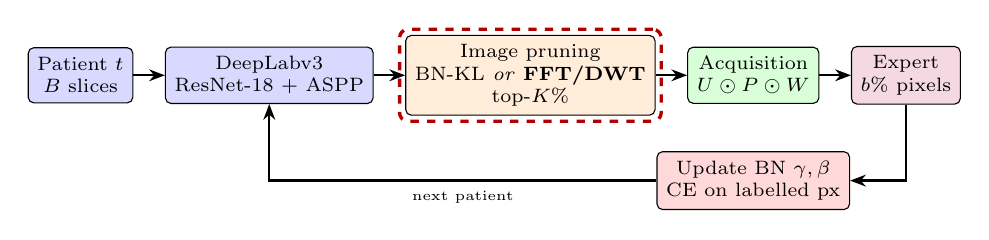
\begin{tikzpicture}[node distance=4mm and 4mm]
  \node[blk=blue] (in) {Patient $t$\\$B$ slices};
  \node[blk=blue, right=of in] (net) {DeepLabv3\\ResNet-18 + ASPP};
  \node[blk=orange, right=of net] (prune) {Image pruning\\BN-KL \emph{or} \textbf{FFT/DWT}\\top-$K\%$};
  \node[blk=green, right=of prune] (acq) {Acquisition\\$U\odot P\odot W$};
  \node[blk=purple, right=of acq] (exp) {Expert\\$b\%$ pixels};
  \node[blk=red, below=6mm of acq] (upd) {Update BN $\gamma,\beta$\\CE on labelled px};
  \draw[arr] (in) -- (net); \draw[arr] (net) -- (prune); \draw[arr] (prune) -- (acq); \draw[arr] (acq) -- (exp);
  \draw[arr] (exp) |- (upd); \draw[arr] (upd) -| node[pos=0.25,below,font=\tiny]{next patient} (net);
  \begin{scope}[on background layer]\node[new, fit=(prune), inner sep=2pt] {};\end{scope}
\end{tikzpicture}
\caption{ODES / FreqODES pipeline for one incoming patient. FreqODES changes only the dashed image-pruning block.}
\label{fig:arch}
\end{figure}

\subsection{Completing the public implementation}
The official repository provides the online loop but not a runnable pipeline. We added: a CHAOS conversion script (DICOM and PNG to per-patient stacks, with slice--label alignment checked by edge correlation); a source-training script; the module \texttt{FFT\_weight\_2.py} imported by the code but not released, re-implemented from Algorithm~2 of the paper; device-agnostic code (CUDA was hard-coded); and two selection fixes (the diversity map was computed but its multiplication was commented out, and a stale variable from a previous slice could replace the current acquisition map). The BN distance was vectorised without changing its value.

\subsection{Dataset and protocol}
We use the 20 MR training cases of CHAOS~\cite{kavur2021chaos}, T1-DUAL sequence: 647 axial slices (26--50 per patient) of $256\times256$ or $288\times288$ pixels, resized to $256\times256$ and min--max normalised per slice. Labels are liver, right kidney, left kidney and spleen plus background. Following the paper, the source model is trained on the IP volumes and the 20 OOP volumes are streamed once, in a fixed order, as 20 online batches; every patient is evaluated right after its own adaptation step. All runs share the same seed (1337), model, budgets and order.

\subsection{Training and adaptation settings}
The DeepLabv3~\cite{chen2017deeplab} model with an ImageNet-initialised ResNet-18 encoder is trained on IP slices for 25 epochs with Adam (learning rate $10^{-3}$, weight decay $10^{-4}$, cosine schedule), batch size 8, cross-entropy plus Dice loss, and random flips, $90^\circ$ rotations and intensity jitter. Adaptation uses Adam with learning rate $10^{-2}$, one step per patient, updating only BN affine parameters; the patch radius is 2 ($5\times5$ patches) and $b=1\%$. The BN score uses 20 augmented copies per slice as in the released code. Experiments ran in PyTorch on an NVIDIA Tesla T4 (Google Colab).

\section{Proposed modification: FreqODES}
\subsection{Frequency-domain shift score}
For a slice $x$ (zero-mean), the \textbf{FFT descriptor} is the vector of log relative energies of $|\mathcal{F}(x)|^2$ in $N_b=16$ concentric radial frequency bands of the centred spectrum. The \textbf{DWT descriptor} is the vector of log relative energies of the sub-bands of a three-level Haar decomposition (LL$_3$ and LH$_l$, HL$_l$, HH$_l$ for $l=1,2,3$). A reference mean $\mu_f$ and standard deviation $\sigma_f$ of each descriptor component are estimated once from 200 random source slices. The shift score of a target slice is the diagonal Mahalanobis distance
\begin{equation}
D_{freq}(x)=\frac{1}{d}\sum_{f=1}^{d}\left(\frac{\phi_f(x)-\mu_f}{\sigma_f}\right)^2 ,
\end{equation}
computed for FFT, DWT, or their average (FFT+DWT). The \textbf{fused} variant combines both criteria after normalising each by its batch maximum: $D=\lambda\hat D_{BN}+(1-\lambda)\hat D_{freq}$; $\lambda=1$ recovers ODES.

\subsection{FreqODES-U: frequency shift times uncertainty}
The first evaluation (Section~\ref{sec:results}) showed that the most frequency-shifted slices are not always the most useful to label. We therefore designed, before running it, a second score that also asks whether the model is struggling: v2 $=\hat D_{freq}\times\hat A\times\hat H$, where $\hat A$ is the fraction of the slice predicted as organ and $\hat H$ is the mean pixel entropy of the softmax prediction, each normalised by its batch maximum, together with the two ablations that drop one factor each. The variant
\begin{equation}
S(x_j)=\hat D_{freq}(x_j)\cdot\hat H(x_j),
\end{equation}
which we call \textbf{FreqODES-U}, performed best. $\hat H$ is computed from the inference prediction that ODES already makes, so the score still needs no extra forward passes. All variants were evaluated with three seeds (1, 2, 12345) and are reported in full.

\subsection{Rationale}
The frequency score uses an explicit, physically interpretable signal---how the image's energy is distributed across spatial frequencies---instead of activation statistics that assume Gaussian channels. It needs no network forward passes and no augmentation, and the descriptors can be visualised to explain each selection. All other ODES stages are untouched, so differences are attributable to the pruning criterion alone.

\section{Results}\label{sec:results}
\subsection{Shift detection}
Figure~\ref{fig:freq} shows that OOP slices have systematically more high-frequency energy than IP slices, in both descriptors. Using the score alone to separate held-out IP slices (10 patients not in the reference) from OOP slices gives ROC-AUC \AUCFFT\ (FFT), \AUCDWT\ (DWT) and \AUCFREQ\ (FFT+DWT). The score also increases monotonically with synthetic Gaussian noise and blur.

\begin{figure}[t]
\centering
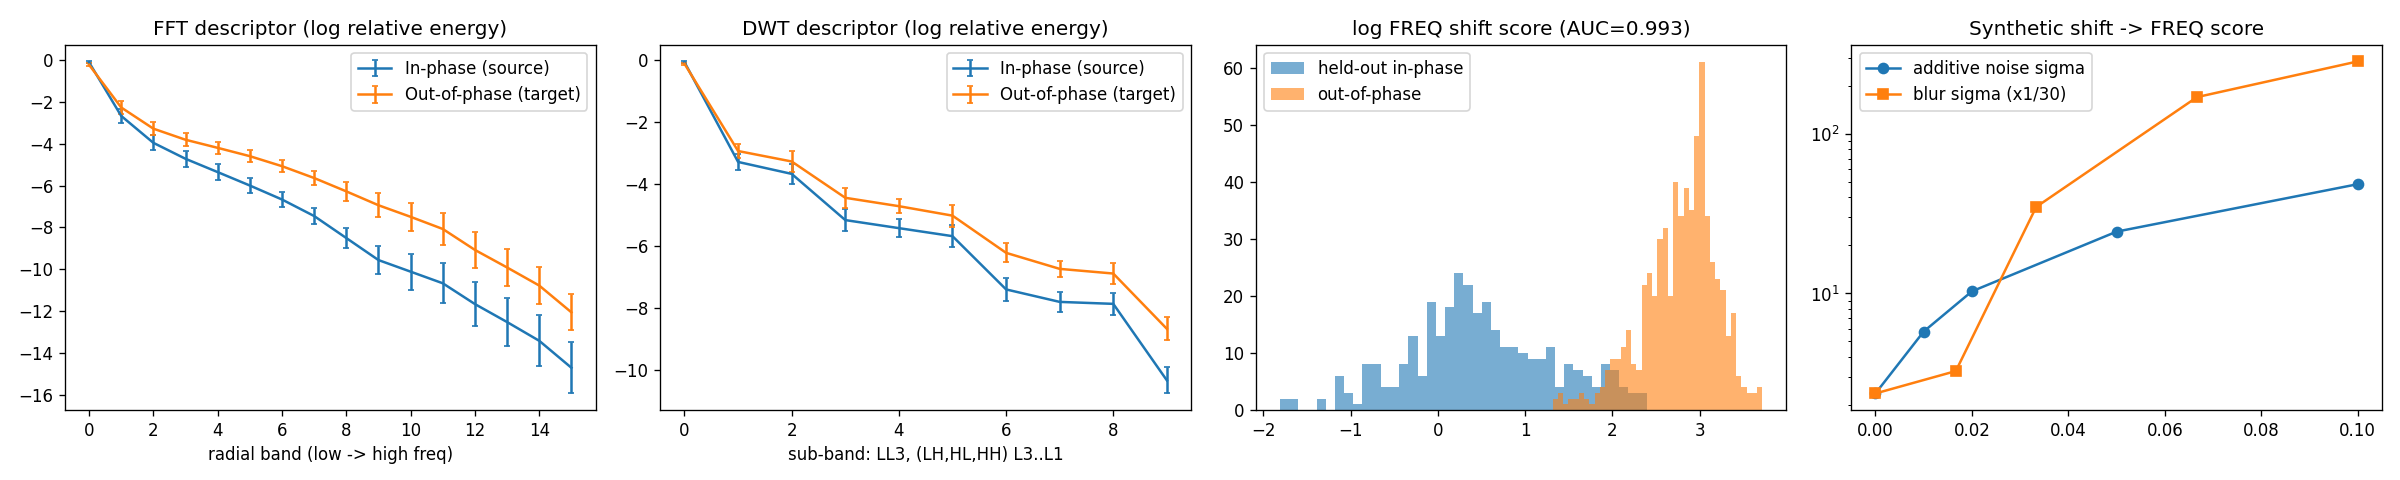
\includegraphics[width=\textwidth]{figures/freq_analysis.png}
\caption{Frequency analysis of CHAOS T1-DUAL. From left: mean FFT radial-band descriptor, mean DWT sub-band descriptor (error bars: std), histogram of the FFT+DWT shift score, and score under synthetic noise and blur.}
\label{fig:freq}
\end{figure}

\subsection{Replication}
Table~\ref{tab:rep} compares our replication with the published results. With all slices annotated we obtain \DODESK\% mean Dice (paper 78.61\%), and the trend over $K$ is reproduced. Our source-only model is close to the paper's (\Dsourceonly\% vs.\ 52.99\%), so the adaptation gain of about 25 Dice points is reproduced; as no source checkpoint or training recipe is published, the remaining organ-level differences (notably the kidneys) most likely come from source training. Fig.~\ref{fig:train} shows the training loss and the per-patient Dice during online adaptation.

\begin{table}[t]
\caption{Replication on CHAOS IP$\rightarrow$OOP ($b=1\%$). Dice per organ and mean Dice / Jaccard (\%). Paper values are from Table~1 of~\cite{islam2025odes}, which does not report Jaccard.}
\label{tab:rep}
\centering\small
\begin{tabular}{llcccccc}
\toprule
Setting & Source & Liver & L.\,kidney & R.\,kidney & Spleen & Mean DSC & Mean IoU \\
\midrule
\multirow{2}{*}{Source only} & Paper & 87.77 & 37.97 & 18.92 & 67.31 & 52.99 & -- \\
 & Ours & \DsourceonlyLiver & \DsourceonlyLK & \DsourceonlyRK & \DsourceonlySpleen & \Dsourceonly & \Jsourceonly \\
\multirow{2}{*}{ODES, $K=100$} & Paper & 88.90 & 72.41 & 74.55 & 78.56 & 78.61 & -- \\
 & Ours & \DODESKLiver & \DODESKLK & \DODESKRK & \DODESKSpleen & \DODESK & \JODESK \\
\multirow{2}{*}{ODES, $K=50$} & Paper & 89.13 & 72.30 & 74.43 & 78.36 & 78.56 & -- \\
 & Ours & \DBNKFiftyLiver & \DBNKFiftyLK & \DBNKFiftyRK & \DBNKFiftySpleen & \DBNKFifty & \JBNKFifty \\
\multirow{2}{*}{ODES, $K=10$} & Paper & 88.41 & 71.45 & 70.22 & 77.12 & 76.80 & -- \\
 & Ours & \DBNKTenLiver & \DBNKTenLK & \DBNKTenRK & \DBNKTenSpleen & \DBNKTen & \JBNKTen \\
\bottomrule
\end{tabular}
\end{table}

\begin{figure}[t]
\centering
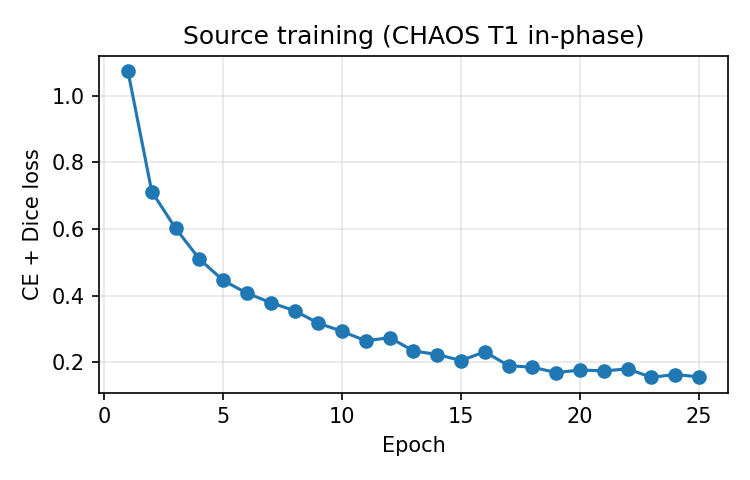
\includegraphics[width=0.42\textwidth]{figures/train_loss.png}\hfill
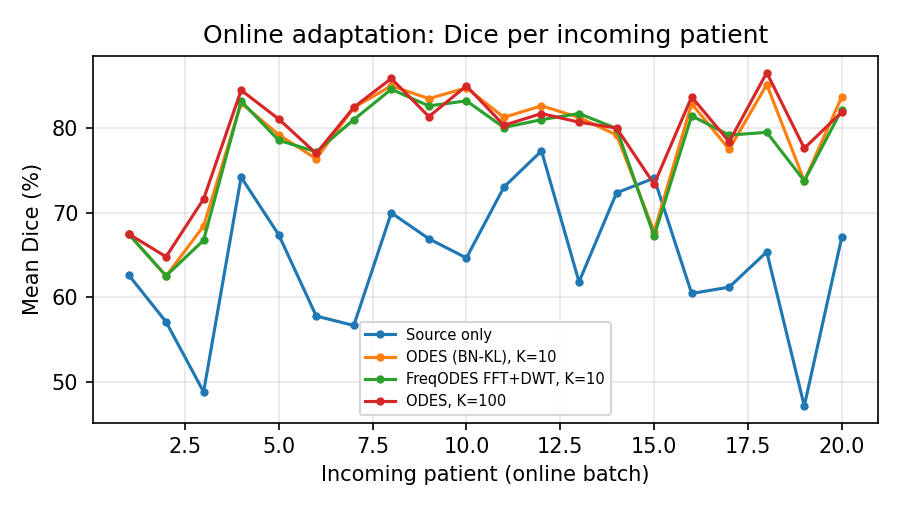
\includegraphics[width=0.54\textwidth]{figures/online_dice.png}
\caption{Left: source training loss. Right: mean Dice of each incoming target patient during online adaptation.}
\label{fig:train}
\end{figure}

\IfFileExists{figures/qualitative.png}{%
\begin{figure}[t]
\centering
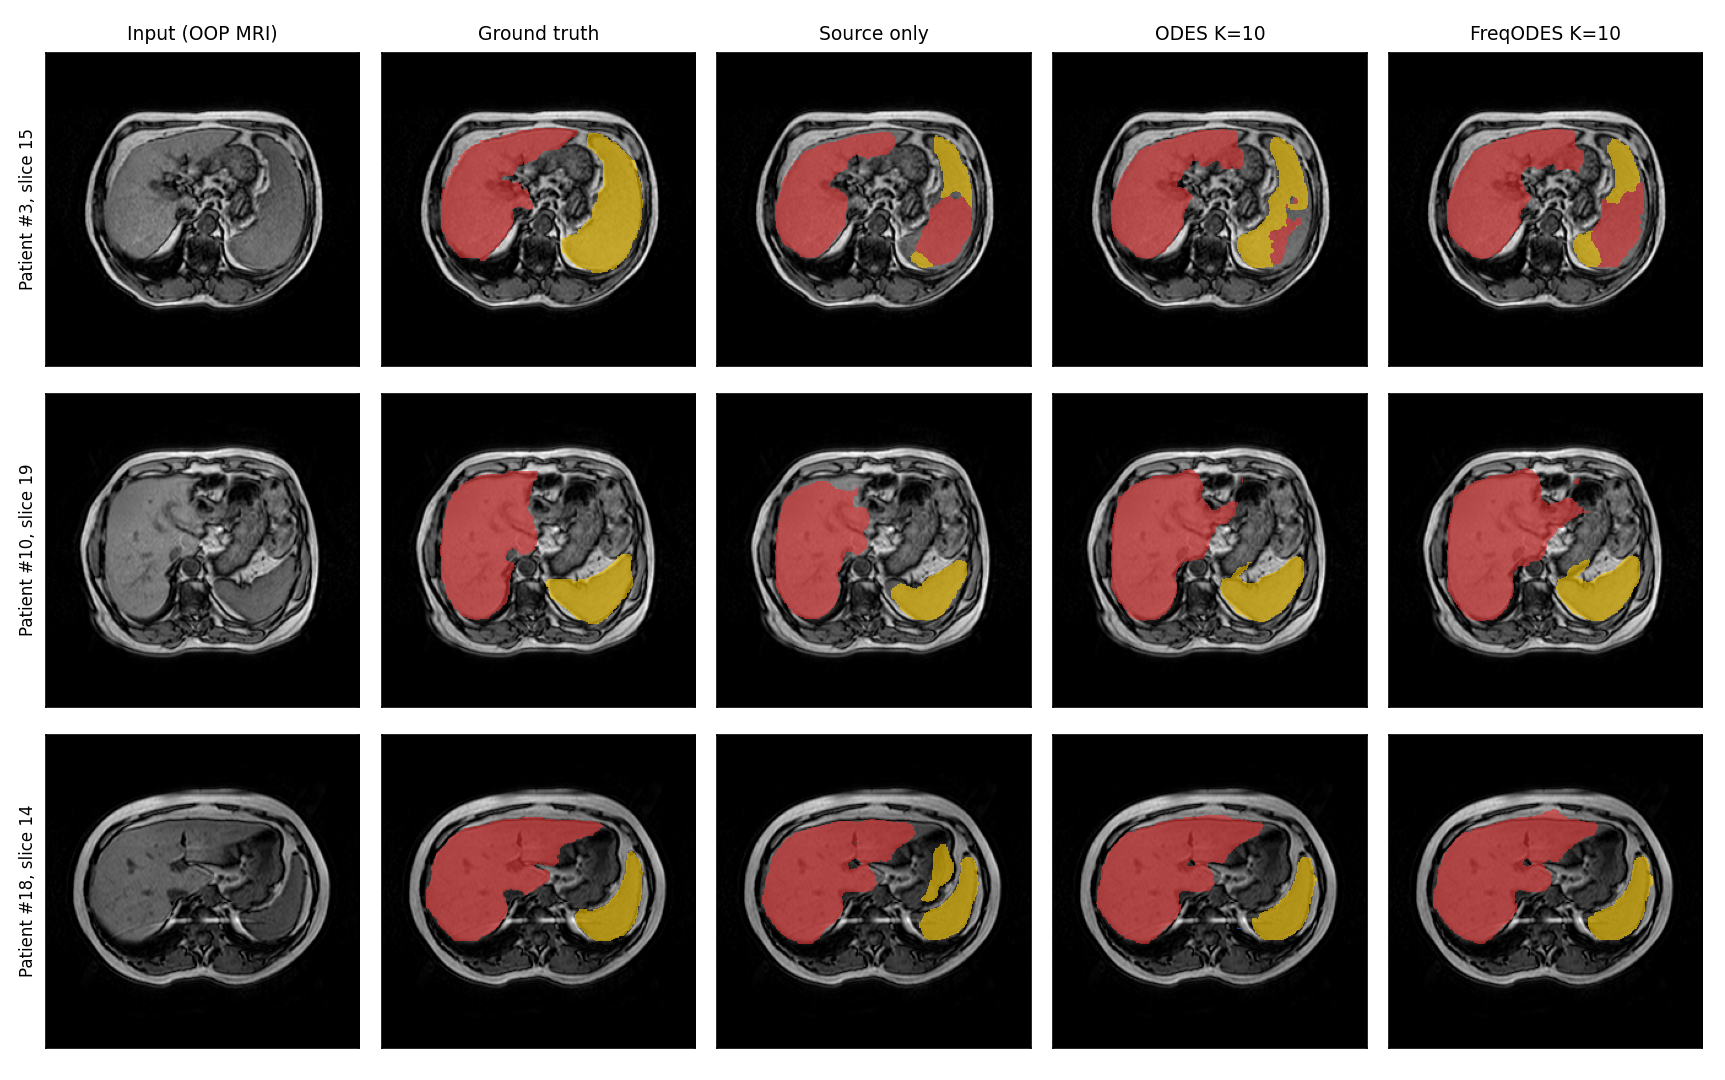
\includegraphics[width=\textwidth]{figures/qualitative.png}
\caption{Qualitative results on three OOP patients: input, ground truth, and predictions of the source model, ODES ($K=10$) and FreqODES ($K=10$). Red: liver; green: right kidney; blue: left kidney; yellow: spleen.}
\label{fig:qual}
\end{figure}}{}

\subsection{ODES versus FreqODES}
Table~\ref{tab:cmp} compares the pruning criteria at equal budget, together with the time of a full online pass over the 20 patients. At $K=50\%$ all criteria are within half a Dice point of annotating every slice; the fused score (\DFUSEDKFiftyLFifty\%, $p=\PFUSEDKFiftyLFifty$) and random pruning are on par with ODES (\DBNKFifty\%), while the pure frequency scores trail by 0.3--0.5 points. At $K=10\%$, the pure frequency scores trail ODES (\DBNKTen\%) by 0.6--0.8 points (significant for FFT and DWT), whereas the fused score with $\lambda=0.25$ (\DFUSEDKTenLQuarter\%) and random pruning (\DRANDOMKTen\%) are not significantly different from ODES. Frequency pruning reduces the online pass from \TBNKTen\,s to \TFREQKTen\,s.

\begin{table}[t]
\caption{Pruning criteria at equal budget ($b=1\%$, same seed). DSC / IoU in \%; $p$: paired Wilcoxon signed-rank test over the 20 patients against ODES at the same $K$; time: full online pass on a T4.}
\label{tab:cmp}
\centering\small
\begin{tabular}{lcccc@{\hskip 5mm}cccc}
\toprule
 & \multicolumn{4}{c}{$K=10\%$} & \multicolumn{4}{c}{$K=50\%$} \\
Pruning & DSC & IoU & $p$ & Time (s) & DSC & IoU & $p$ & Time (s) \\
\midrule
BN-KL (ODES) & \DBNKTen & \JBNKTen & -- & \TBNKTen & \DBNKFifty & \JBNKFifty & -- & \TBNKFifty \\
FFT & \DFFTKTen & \JFFTKTen & \PFFTKTen & \TFFTKTen & \DFFTKFifty & \JFFTKFifty & \PFFTKFifty & \TFFTKFifty \\
DWT & \DDWTKTen & \JDWTKTen & \PDWTKTen & \TDWTKTen & \DDWTKFifty & \JDWTKFifty & \PDWTKFifty & \TDWTKFifty \\
FFT+DWT & \DFREQKTen & \JFREQKTen & \PFREQKTen & \TFREQKTen & \DFREQKFifty & \JFREQKFifty & \PFREQKFifty & \TFREQKFifty \\
Fused ($\lambda=0.5$) & \DFUSEDKTenLFifty & \JFUSEDKTenLFifty & \PFUSEDKTenLFifty & \TFUSEDKTenLFifty & \DFUSEDKFiftyLFifty & \JFUSEDKFiftyLFifty & \PFUSEDKFiftyLFifty & \TFUSEDKFiftyLFifty \\
Random & \DRANDOMKTen & \JRANDOMKTen & \PRANDOMKTen & \TRANDOMKTen & \DRANDOMKFifty & \JRANDOMKFifty & \PRANDOMKFifty & \TRANDOMKFifty \\
\bottomrule
\end{tabular}
\end{table}

\subsection{Ablation studies}
Table~\ref{tab:abl} reports the pruning $\times$ diversity-weighting ablation of the paper's Table~3 and the fusion-weight sweep. Diversity weighting changes the mean Dice by at most 0.2 points in our runs, much less than the gains reported in the paper. In the fusion sweep the pure frequency score is lowest; any amount of BN information brings the result back to the level of ODES, and $\lambda=0.25$ gives the best value (\DFUSEDKTenLQuarter\%), although the differences between $\lambda>0$ settings are within run-to-run noise.

\begin{table}[t]
\caption{Ablations at $K=10\%$ (mean Dice, \%). Left: image pruning $\times$ diversity weighting (D.W.). Right: fusion weight $\lambda$.}
\label{tab:abl}
\centering\small
\begin{tabular}{lcc}
\toprule
Pruning & D.W. off & D.W. on \\
\midrule
BN-KL (ODES) & \DBNKTennoDW & \DBNKTen \\
FFT+DWT (ours) & \DFREQKTennoDW & \DFREQKTen \\
Random & \DRANDOMKTennoDW & \DRANDOMKTen \\
Paper: BN-KL / random & 75.88 / 74.32 & 76.80 / 75.41 \\
\bottomrule
\end{tabular}\hspace{8mm}
\begin{tabular}{lc}
\toprule
$\lambda$ & Mean DSC \\
\midrule
0 (frequency only) & \DFREQKTen \\
0.25 & \DFUSEDKTenLQuarter \\
0.5 & \DFUSEDKTenLFifty \\
0.75 & \DFUSEDKTenLThreeQ \\
1 (BN only = ODES) & \DBNKTen \\
\bottomrule
\end{tabular}
\end{table}

\begin{figure}[t]
\centering
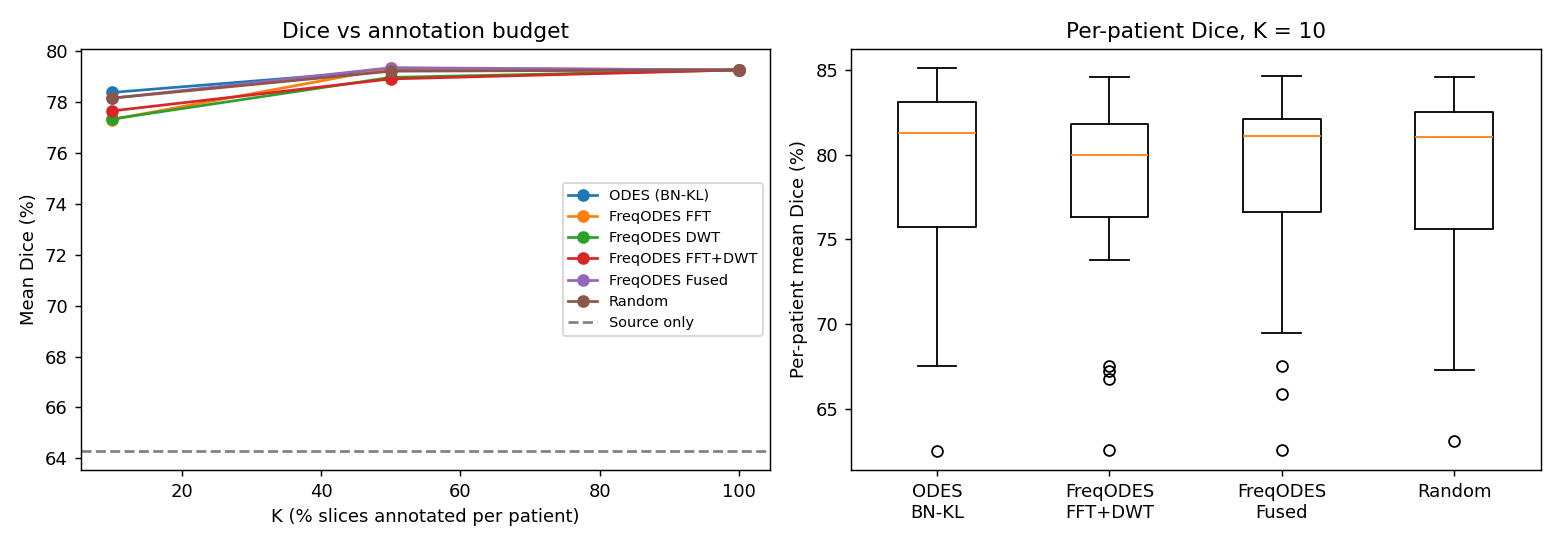
\includegraphics[width=0.95\textwidth]{figures/dice_vs_budget.png}
\caption{Left: mean Dice versus the share $K$ of slices annotated, for each pruning criterion. Right: distribution of per-patient Dice at $K=10\%$.}
\label{fig:budget}
\end{figure}

\subsection{FreqODES-U over three seeds}
Table~\ref{tab:v2} and Fig.~\ref{fig:v2} report all v2 variants over three seeds. With 10\% of slices annotated, FreqODES-U reaches \VFeTenMean\% mean Dice against \VBnTenMean\% for ODES ($\Delta=\VFeTenDiff$, $p=\VFeTenP$ over 60 paired patient-runs) and is better on every seed (\VFeTenSa, \VFeTenSb, \VFeTenSc\ vs.\ \VBnTenSa, \VBnTenSb, \VBnTenSc). It is also far more stable across seeds (standard deviation \VFeTenStd\ vs.\ \VBnTenStd) and about one third faster. The pre-planned v2 with the organ-area term (\VFvTenMean\%) and the area-only ablation (\VFaTenMean\%) are not significantly different from ODES, so the area factor does not help. With 50\% of slices annotated ODES remains best (\VBnFiftyMean\% vs.\ \VFeFiftyMean\%, $p=\VFeFiftyP$). The single-seed results of the previous subsections differ from these averages by up to about one Dice point, which shows why several seeds are needed for differences of this size.

\begin{table}[t]
\caption{FreqODES-U and its variants over three seeds. Mean Dice $\pm$ standard deviation (\%); $\Delta$ and $p$: paired Wilcoxon signed-rank test against ODES over 60 patient-runs; time: full online pass on a T4.}
\label{tab:v2}
\centering\small
\begin{tabular}{lcccc@{\hskip 5mm}ccc}
\toprule
 & \multicolumn{4}{c}{$K=10\%$} & \multicolumn{3}{c}{$K=50\%$} \\
Selection score & DSC & $\Delta$ / $p$ & IoU & Time (s) & DSC & $\Delta$ / $p$ & IoU \\
\midrule
ODES (BN-KL) & \VBnTenMean$\pm$\VBnTenStd & -- & \VBnTenIoU & \VBnTenTime & \VBnFiftyMean$\pm$\VBnFiftyStd & -- & \VBnFiftyIoU \\
v1: frequency & \VFqTenMean$\pm$\VFqTenStd & \VFqTenDiff\ / \VFqTenP & \VFqTenIoU & \VFqTenTime & \VFqFiftyMean$\pm$\VFqFiftyStd & \VFqFiftyDiff\ / \VFqFiftyP & \VFqFiftyIoU \\
v2: freq $\times$ area $\times$ unc. & \VFvTenMean$\pm$\VFvTenStd & \VFvTenDiff\ / \VFvTenP & \VFvTenIoU & \VFvTenTime & \VFvFiftyMean$\pm$\VFvFiftyStd & \VFvFiftyDiff\ / \VFvFiftyP & \VFvFiftyIoU \\
freq $\times$ area & \VFaTenMean$\pm$\VFaTenStd & \VFaTenDiff\ / \VFaTenP & \VFaTenIoU & \VFaTenTime & -- & -- & -- \\
\textbf{FreqODES-U} & \textbf{\VFeTenMean}$\pm$\VFeTenStd & \VFeTenDiff\ / \VFeTenP & \VFeTenIoU & \VFeTenTime & \VFeFiftyMean$\pm$\VFeFiftyStd & \VFeFiftyDiff\ / \VFeFiftyP & \VFeFiftyIoU \\
Random & \VRdTenMean$\pm$\VRdTenStd & \VRdTenDiff\ / \VRdTenP & \VRdTenIoU & \VRdTenTime & \VRdFiftyMean$\pm$\VRdFiftyStd & \VRdFiftyDiff\ / \VRdFiftyP & \VRdFiftyIoU \\
\bottomrule
\end{tabular}
\end{table}

\begin{figure}[t]
\centering
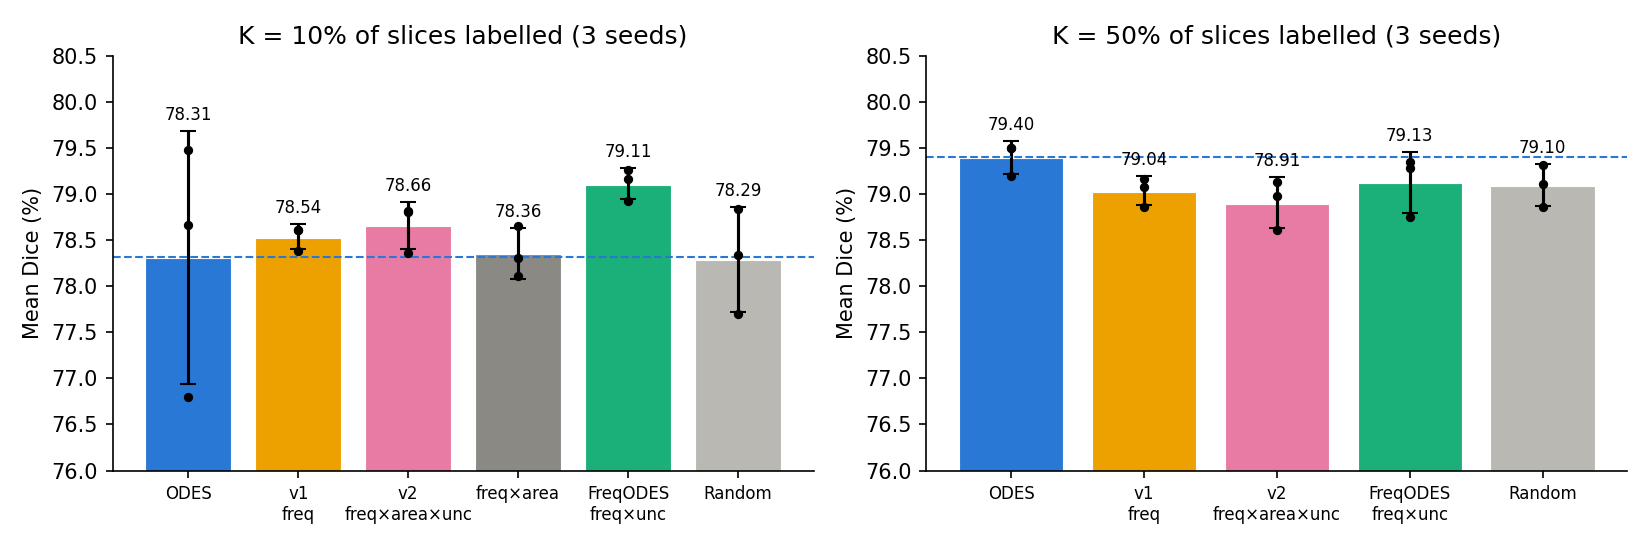
\includegraphics[width=0.95\textwidth]{figures/v2_results.png}
\caption{Three-seed results. Bars: mean Dice; error bars: standard deviation; dots: individual seeds; dashed line: ODES.}
\label{fig:v2}
\end{figure}

\section{Discussion}
Used alone, the frequency score did not improve segmentation accuracy, although it is a better and cheaper detector of domain shift; fused with the BN score it only matched ODES. We see four reasons.
\textbf{(1) Objective mismatch.} The frequency score answers ``how different is this slice from the source?'', whereas pruning should answer ``which labels will most improve the model?''. The slices with the most unusual spectra are often at the ends of the volume, where organs are small or absent; labelling them teaches the BN layers little. The BN score measures what the \emph{network} finds unusual, which correlates better with its errors.
\textbf{(2) Global, homogeneous shift.} IP$\rightarrow$OOP is a sequence change that affects every slice, so almost all target slices are ``shifted'' and the useful information is in the ranking among them; this is also why random pruning is competitive.
\textbf{(3) Small effect sizes.} Differences between criteria are about one Dice point, so a single seed and 20 patients limit the conclusions; we report paired tests rather than claim small gains.
\textbf{(4) Saturation.} All adapted variants lie between 78 and 80 Dice, close to the result with every slice annotated, so the pruning criterion has little room to make a difference on this pair.
Reason (1) suggested the fix that FreqODES-U implements: weighting the shift by the model's uncertainty keeps the image-level signal but favours slices on which the network is actually unsure, and this beats ODES at the 10\% budget. That the organ-area term did not help suggests that uncertainty already captures what makes a slice informative. At the 50\% budget, half of each volume is labelled anyway and the selection criterion matters less, which is consistent with ODES keeping a small lead there.
\textbf{Limitations.} FreqODES-U was the best of the planned v2 ablations rather than the planned score itself, so its advantage should be confirmed on further data; we report all variants to make this transparent. The evaluation uses one adaptation pair (CHAOS IP$\rightarrow$OOP), 20 patients and three seeds, and the expert is simulated with ground-truth labels. Next steps are CHAOS$\rightarrow$DUKE and BMC$\rightarrow$RUNMC, where shifts are larger and more heterogeneous, more seeds and stream orders, and computing spectra inside organ regions of interest.

\section{Conclusion}
We reproduced ODES on CHAOS T1-DUAL IP$\rightarrow$OOP after completing its public implementation, obtaining results close to the published ones. We proposed FreqODES, which ranks slices for expert annotation with an FFT/DWT frequency-domain shift score. It detects the domain shift almost perfectly and is about one third faster, but shift magnitude alone is an incomplete proxy for annotation value. Combining it with model uncertainty, FreqODES-U outperforms ODES when only 10\% of slices are annotated (\VFeTenMean\% vs.\ \VBnTenMean\% Dice over three seeds, $p=\VFeTenP$), with lower variance and lower cost, while ODES stays slightly better at a 50\% budget.

\section*{Code and data availability}
Code, configuration, logs and result files: \url{https://github.com/Vishnu868/FreqODES}. CHAOS is available from Zenodo (record 3431873).

\section*{CRediT authorship contribution statement}
Both authors took part in every stage of the project. \textbf{Vishnu Vardhan:} Software, Data curation, Investigation, Methodology (environment set-up, CHAOS preprocessing, completion of the ODES code, source-model training and replication, implementation of the FFT/DWT score and FreqODES-U, GPU experiments, code repository). \textbf{Nithya Sai:} Conceptualization, Formal analysis, Validation, Visualization, Writing -- original draft (literature survey and proposal, frequency analysis of in-phase vs.\ out-of-phase images, v2 design and ablation plan, three-seed evaluation, statistical analysis, figures, slides and report).
\section*{Acknowledgement}
The ODES software used in this work was created by Amit Roy-Chowdhury and members of the Vision and Learning Group at UCR. \copyright\ 2025 UCR.

\bibliographystyle{cas-model2-names}
\bibliography{refs}

\end{document}
